\chapter{Design Principles of Software-defined Storage}
\label{chap:design_principles}

This chapter derives the design
principles of SDS using real-world observations of contemporary
system-of-systems applications.
It describes the components that make up an SDS system
and shows how they work together to preserve end-to-end semantics while
preserving organizational autonomy.

\section{Overview}

The design principles for wide-area software-defined storage are rooted in 
observations of three ``tussle spaces''~\cite{david-clark-tussle-spaces}.
These are (1) the cloud services that host and serve the raw
bytes, (2) the end-to-end storage semantics, and (3) the trust
relationships between organizations, their users, and cloud services.
A well-designed SDS system helps application developers efficiently accommodate tussles
in all three of these domains.

\subsection{Semantic Tussle Spaces}

It may not be obvious that end-to-end storage semantics warrant their own tussle
space, distinct from the cloud services and applications.  Why not simply
design applications to be portable?  Is there a system-of-systems application
development methodology that allows applications to be written once, and be made
to run on any services with only a small amount of work?

This thesis argues that focusing only on application portability is
inefficient---it takes a lot of work to build portable system-of-systems
applications with today's methodologies.
Today, the cost of porting $m$ applications to $n$ services
would require $O(mn)$ patches.  This is true even if developers share their
patches, since getting a patch to work with one application can require completely
re-writing it to work with another application.

It is unlikely that this situation will improve on its own,
since developers are incentivized to ship code that \emph{works
today} as opposed to code that is portable to unspecified systems at unspecified
times in the future.  Moreover, the business models of cloud services
depend on customers continuously paying for the service, which removes the
incentive to help make applications portable to their competitors.
Even if portability was a desireable and achievable design goal from the get-go,
getting $m$ applications to adopt a new service's behavior would still at best
require $O(m)$ man-hours, since each application would need to be modified.

SDS reframes the problem of portability as a problem with isolating
both the individual service's semantics and the desired end-to-end storage
semantics from the application.  By treating the set of application
end-to-end semantics as their own tussle space, SDS frees the developer from
having to port the application to each service.  Instead, a developer simply
ports the service to the SDS system, and the SDS system overlays the desired
end-to-end semantics ``on top'' of them.  Then, all current and future SDS
applications would be able to use the service \emph{without} modification.
The amount of work to port $m$ applications to $n$ services with a SDS system is reduced to
$O(m+n)$.

\subsection{Trust Tussle Spaces}

Trust relationships are not static, and system-of-systems applications need a
way to accomodate changes in trust.  However, the application needs a way to do
so without compromising \emph{any} organization's autonomy.  
The two approaches today---federations and open-membership
architectures---do not fully accomodate trust tussles.  They 
either sacrifice organizational autonomy (federations) or sacrifice 
the flexibility needed to accomodate new trust models (open-membership
architectures).

In federations, each organization promises to adhere to a
``common ground'' data-hosting policy that allows them to interoperate.
This way, users that trust one organization can trust other member organizations
and their users to preserve their policies.
For example, the operators of a set of organizations may agree to use a
single-sign-on (SSO) system to authorize computers from different organizations
to access sensitive data.  As another example, a set of organizations may agree
to use a common data format and API for sharing data with one another (such as
putting their data servers behind an API endpoint that emulates Amazon S3).

While federations help organizations accommodate
tussles in trust relationships, they impose high and unfair coordinaton costs
that impinge on one or more organizations' decision-making.  The problem is 
that organization administrators must regularly coordinate to adapt
to changing trust relationships (imposing a high cost), and do so in a way that
favors certain organizations over others (removing fairness).  For example,
federations governed by in-person meetings exclude individuals who cannot
travel easily or live in different timezones.
As another example, federations whose coordination occurs in English
penalizes non-English-speaking participants.  The unfairness of the
coordination cost distribution is fundamentally a social problem, and is beyond
the scope of this thesis to address.

Open-membership architectures attempt to accommodate tussles in trust
relationships in a more fair way by embedding all of the coordination logic to do so in the
application protocol itself.  The rationale is
that this reduces the need for organization administrators to coordinate
out-of-band.  Instead, the act of participating in the system gives
each organization the ability to set its own policies for interacting with other
nodes.  Examples systems that follow this architecture include peer-to-peer file sharing
(like BitTorrent~\cite{bittorrent}, Shark~\cite{shark}, and Vanish~\cite{vanish})
and cryptocurrencies (like Bitcoin~\cite{bitcoin} and Ethereum~\cite{ethereum}).

The difficulty with the open-membership approach is that
it makes it difficult to upgrade the application beyond the scope of the
protocol.  This makes it hard to accomodate new types of trust relationships.
The lack of out-of-band coordination between organization
administrators means that developers forgo the ability to significantly change the
system once deployed.  Attempting to introduce a backwards-incompatible change to the
application is tatamount to creating a whole new application.  For example,
the Bitcoin Cash cryptocurrency~\cite{bcash} split off from the Bitcoin
cryptocurrency due to a disagreement in the system's block size (a one-line code
change) after over two years of infighting.

The SDS approach to accommodating tussles in trust relationships is to leverage
an open-membership system to \emph{bootstrap} trust between
users and organizations (Section~\ref{sec:chap2-ssi}).  Users and
organizations leverage the open-membership system to exchange public keys, and
establish end-to-end confidential and authenticated communication channels.
This lets organizations establish trust relationships unilaterally while
avoiding the high-overhead coordination problems of a
federation (preserving autonomy).
It also helps developers avoid getting locked into an un-upgradeable platform,
since the nature of the trust relationships is decoupled from the
open-membership system used to establish them (preserving flexibility).

\subsection{Design Objectives}

Applications not only need to work with existing cloud services, but also with
any \emph{future} cloud services that may be developed after the application is
built and deployed.  The developer must be able to use any services they want,
with minimal switching costs.  This leads to the first design objective for a SDS
system:
\\
\\
\noindent{\textbf{Objective 1}}: \emph{Once developed, an application must be
able to use any current or future 
cloud service to host data without changing its end-to-end storage semantics.}
\\
\\
At the same time, a developer may want to stop using a storage system that was
previously in use.  The data must nevertheless remain accessible, and subject to
the organizations' policies.

For example, the application developer may discover that the business logic needs stronger
consistency guarantees than the cloud services can offer.  The developer cannot
simply move to a different service on a whim, since all of the data is hosted 
on the current services.  At the same time, the developer cannot be expected
to rewrite the application to keep using it with its weak consistency model.

This leads to the second design objective for a SDS system:
\\
\\
\noindent{\textbf{Objective 2}}: \emph{Once chosen to host data, a cloud service
must remain usable by the application regardless of any future changes to the
application's end-to-end storage semantics.}
\\
\\
All the while, the trust relationships between organizations, their users, and
their chosen services determine how applications are permitted to
interact with its data.  If organizations and users can communicate securely,
it can be shown that they only need to trust cloud services with
keeping their data available.  Other policies can be enforced
in software outside of the service (Section~\ref{sec:aggregation-driver-model}).

However, this leaves open the question of how users and
organizations establish trust in one another in the first place.  They must
establish trust relationships \emph{outside} of the application, since they need
to trust each other before any cross-organization data interactions can occur.  Organizations should
not be expected to send or receive data from untrusted sources, since that
infringes on their autonomy.

This leads to the third SDS design objective:
\\
\\
\noindent{\textbf{Objective 3}}: \emph{Users and organizations must be free to
establish trust in one another independent of the
applications and cloud services they use.}
\\
\\
If this objective is met, then it becomes possible for organizations to
securely identify with whom they will share data.  Once they can do this,
they can go on to define non-trivial data-hosting policies based on non-trivial
application-specific trust models.

Organizations would not need the application developer to be aware
of their trust relationships.  Organizations would only need the developer to
ensure that their data-hosting policies (which encompass their trust
relationships) get enforced.

Identifying and authenticating other organizations and their users
is the first step to implementing policy-enforcement mechanisms.
The second step is to ensure that the organization can unilaterally
designate which organization(s) can be trusted to run them.
Once these preconditions are met, then it is up to the SDS system to ensure that the right
policy enforcement mechanisms are invoked by the right organizations during a read or write.

This leads to the final SDS design objective:
\\
\\
\noindent{\textbf{Objective 4}}: \emph{An organization's data-hosting policies
must be enforced independently of applications and cloud services.}
\\
\\
The remainder of this chapter shows how these objectives sculpt the design space
for SDS systems.  It concludes by distilling the design space into a set of
design principles for SDS system design and implementation.

\section{Requirements}

\begin{figure}[h]
   \caption{Logical representation of a wide-area SDS system.  The SDS system
   is a cross-organization intermediate layer that connects services to
   applications via distinct interfaces.}
   \centering
   \includegraphics[width=0.9\textwidth,page=2]{figures/dissertation-figures}
   \label{fig:chap2-sds-overview}
\end{figure}

At a high-level, an SDS system is a logical ``hub'' between applications and
services that spans multiple organizations (Figure~\ref{fig:chap2-sds-overview}). 
The hub takes reads and writes from the application, processes them
according to application-defined semantics, and loads and stores the resulting
data to the underlying storage systems.
It offers two interfaces:  a \emph{service interface} through which it interacts with
services on the applications' behalf, and an \emph{application interface} through
which applications interact with data and define their desired storage
semantics.

\subsection{Service Interface}

The service interface is similar to existing work on service compatibility
libraries.  In particular, the interface allows SDS to divide the set of
services into three distinct classes, where each class has a driver model that
when implemented will enable applications to use it.  The service driver models
enable the following:

\begin{itemize}
   \item \textbf{Treat cloud storage as a write-once read-many medium}.  The set of cloud storage
      services in use must collectively appear to be a single
      read/write storage medium with a uniform access interface.  A given record
      is written no more than once, but read many times.
   \item \textbf{Treat data sets as read-only medium}.  The set of individual
      data sets must collectively appear to be a single read-only
      storage medium with a uniform access interface.
   \item \textbf{Treat CDNs as a write-through cache}.  The set of CDNs
      must appear as a write-coherent cache.  Despite their transparent presence
      on the read path, they cannot be allowed to affect the end-to-end storage
      semantics.
\end{itemize}


\begin{figure}[h]
   \caption{Service and aggregation drivers in an SDS system.  Aggregation
   drivers span multiple organizations and route application reads and writes to
   one or more service drivers.}
   \centering
   \includegraphics[width=0.9\textwidth,page=3]{figures/dissertation-figures}
   \label{fig:chap2-driver-overview}
\end{figure}

Logically speaking, service drivers run at the service-facing ``bottom'' of the
SDS ``hub'' (Figure~\ref{fig:chap2-driver-overview}).
They handle only the data meant to be hosted on the service.  The SDS system may
instantiate multiple copies of the service drivers in order to handle higher
load or keep applications isolated from one another.

\subsection{Application Interface}

Developers need to be able to specify
end-to-end storage semantics across an aggregation of services
in a multi-user setting.  To enable this,
SDS offers a separate type of driver model called an ``aggregation
driver.''

There is one aggregation driver per application.  Logically speaking, it runs at
the ``top'' of the SDS ``hub'' (Figure~\ref{fig:chap2-driver-overview})
and mediates all requests between users and
service drivers (note that this thesis does not
distinguish between users and the application clients
they run).  It mediates interactions in terms of \emph{which user} issues the
interaction, \emph{which operation} is requested, \emph{which data
record} is affected, and \emph{which network host} is originating the request.

The high-level idea behind having two driver classes is that once a service has an appropriate service driver,
it can be ``plugged into'' the SDS system such that existing aggregation drivers
can use it immediately.  An aggregation driver implements the application's desired end-to-end storage
semantics, and translates
application-level requests into requests understood by the service driver.  These
requests are issued such that their execution
by service drivers delivers the desired end-to-end behavior.  This reframes the
costs of porting applications to services:

\begin{itemize}
    \item For the cost of writing only the application-specific
aggregation drivers, a new application can be made
compatible with all existing and future services with no modification.
    \item For the cost of writing only the service-specific SDS driver, a new
service can be made compatible with all existing and future applications.
\end{itemize}

In other words, the cost of porting $m$ applications to $n$ services can be
reduced from $O(mn)$ to $O(m+n)$.

To realize this cost savings, many applications will share an SDS system.  Aggregation and service drivers
will be \emph{decoupled} from the applications---they will be
developed independently of one another, and independently of the
application itself.  Both types of drivers can be re-used by new applications.

\subsection{Data and Control Planes}

The interactions between SDS components are characterized in terms a data plane and a control plane.
The \emph{data plane}'s job
is to ensure all-to-all connectivity between users and services.
It moves the raw bytes between them, but with no concern for
application-specific semantics.  It includes the service-facing interface, the
service drivers, and the data formatting, serialization, and transmission
logic.

The \emph{control plane} implements each application's
storage semantics by acting as a governor for the data plane.
It runs an application's aggregation driver 
to constrain how each of its users interact with the data plane.

The data plane is shared by all applications and all services, and implements a
common data-sharing interface via a fully-connected bidirectional communication graph.
Every node in an SDS-powered application can send and receive data-plane
messages to every other node.  The control-plane defines the behavior of the
system insofar as what messages get sent while processing application I/O, and how they are
transformed and routed to and from the underlying services.

\section{Data Plane}

The SDS data plane organizes data into units called \emph{chunks}.  Chunks form
the basis of all data within SDS, and constitute a ``data plane narrow waist'' between 
a multitude of service drivers below and a multitude of aggregation drivers
above.  Chunks have the following properties in SDS:

\begin{itemize}
    \item Every piece of data in SDS is made of one or more chunks.
    \item Each chunk is immutable.
    \item Each chunk has a globally-unique identifier.
\end{itemize}

The data plane ensures that each chunk belonging to a particular application
is addressable (but not necessarily resolvable) by every process connected to it.
If the aggregation driver logic allows it, each application
endpoint can resolve and download chunks created by other processes in the same
application.

\begin{figure}[h]
   \caption{The narrow waist in the SDS data plane.  The aggregation driver
   translates application-level storage requests into operations on manifests
   and chunks, and service drivers implement simple \textit{create},
   \textit{update}, and \textit{delete} operations on chunks using existing
   service interfaces.}
   \centering
   \includegraphics[width=0.9\textwidth,page=4]{figures/dissertation-figures}
   \label{fig:chap2-narrow-waist}
\end{figure}

At the service driver level, the SDS
system provides operations to \texttt{create}, \texttt{read}, and
\texttt{delete} chunks.  Service drivers execute the requisite protocols
and data transformations to
marshal chunks back and forth to their respective services.

At a layer above the service drivers but beneath aggregation drivers, SDS
groups chunks that belong to the same piece of application data using two specialied
chunk types:  a \emph{block} and a \emph{manifest}.  A block is simply a data
container with a known length.  A manifest identifies a sequence of blocks.
They constitute the ``narrow waist'' of an SDS system's data plane
(Figure~\ref{fig:chap2-narrow-waist}).

Blocks and manifests provide just enough information define a
set of generic operations for manipulating application data, but
without mandating a particular data representation or access interface.
Specifically, they allow a SDS system to define data-plane operations on
application data in terms of the chunks that make them up:

\begin{itemize}
   \item \textbf{Reading data}.  To read a piece of application data, a SDS node locates
    its manifest, fetches it, and then fetches the blocks listed within it.

   \item \textbf{Creating data}.  To write a new piece of data, a SDS node replicates
    its set of chunks and a manifest that contains them.

   \item \textbf{Updating data}.  Modifying an existing
    piece of application data is done by creating blocks with the modified data,
    creating a new manifest with the ``latest'' sequence of blocks, and deleting
    blocks that contain overwritten data.

   \item \textbf{Deleting data}.  Deleting the data is done by
    deleting its manifest and blocks.  Subsequent reads on the manifest and
    blocks will fail.
\end{itemize}

These operations are what allow the SDS system to implement end-to-end
guarantees with higher-level aggregation drivers without having to interface
directly with services.  SDS clients translate application-level data
operations into one or more of these operations.

A key advantage of this protocol is that it gives service drivers insight as to whether or not a
chunk is a block or a manifest, as well as insight on which application-level
datum is being processed.  Developers are encouraged to exploit this in practice to implement
service drivers to transparently carry out both chunk-level and application
data-level optimizations like de-duplication, compression, batch-writes,
defragmentation, and so on.

\subsection{Data Discovery and Indexing}

Ensuring that chunks are globally-addressable requires maintaining a global
chunk inventory so other SDS processes can discover them.  Any time a user creates,
updates, or deletes data, it creates a new manifest
with a new globally-unique identifier.  In order to read the data, a reader
needs to discover the new manifest identifier and the set of SDS-connected
processes that can serve it.  This responsibility is fulfilled by a data plane
subsystem called the metadata service.

\begin{figure}[h]
   \caption{SDS Metadata Service.  The MS resolves names to their current
   manifests, and allows gateways to update the name/manifest binding.
   Manifests are stored in the underlying cloud services, and
   point to the set of blocks that make up the datum.}
   \centering
   \includegraphics[width=0.9\textwidth,page=5]{figures/dissertation-figures}
   \label{fig:chap2-metadata-service}
\end{figure}

The \emph{Metadata Service} (MS) helps users discover the
availability of new chunks, announce the existence of chunks they create, and
identify which SDS-connected processes that can serve a chunk
(Figure~\ref{fig:chap2-metadata-service}).
There is one MS per SDS instance, and
applications share the MS as part of sharing the SDS deployment.

The MS implements an indexing service for manifests.  It binds an unchanging
application-chosen name to a datum's ``latest'' manifest
identifier, and stores hints for discovering the SDS-connected processes that can serve it.
Writers set the manifest identifier and discovery hints 
for a name when they write to the datum.
Readers resolve the datum's identifier to the ``latest'' manifest identifier,
and then proceed to query the MS for the list of processes that can serve its
chunk (e.g. by asking for their network addresses).

\subsubsection{Name Consistency}

The consistency model of the MS's name/identifier mappings determines the \emph{default}
consistency model for an SDS's data.
In Syndicate, for example, the MS offers
per-name sequential consistency.  Once a writer successfully updates the manifest
identifier for a name, all subsequent reads on the name will return the new
identifier.

SDS supports different consistency models in part by allowing the
developer-supplied aggregation driver to decide exactly when to update
the manifest identifier as part of an on-going read or write.
This is enabled through the aggregate driver programming model,
described in Section~\ref{sec:aggregation-driver-model}.

\subsubsection{Service Discovery}

In addition to naming manifests, the MS remembers which processes
(i.e. which host/port pairs) are able to serve the manifest and block chunks.
This information is conveyed by the writer when announcing a new manifest,
and given to readers when querying manifests.

The MS also plays a role in deploying service and aggregation drivers.  The
developer uploads new code to the MS, and the MS ensures that the new drivers
are used to service all subsequent read and write requests.  This is described
in detail in Section~\ref{sec:view-changes}.

\subsubsection{Policy Enforcement}

Due to the roles the MS plays in a SDS system, it is important to consider
which organization or organizations run it.  The design of the MS must not infringe on
each organization's autonomy---it must respect all organization's data hosting
policies.

This requirement allows for two possible MS designs.  On the one hand,
the MS can be designed to be distributed across each organization such that each
organization controls the service discovery and naming for its data and
services.  In this design, organizational autonomy is preserved because each
organization mediates all accesss to its metadata and service discovery
information.  This is the design strategy taken by
Gaia's MS.

On the other hand, the MS can be designed such that each organization
places no more trust in its ability to enforce data hosting policies
than it than it already does in its chosen cloud services.  In other words, the
mS could run in an external cloud service, and would only be trusted
with data availability.  This is the design strategy taken by Syndicate's MS.

\section{Control Plane}

An aggregation driver can be thought of as a program running in the SDS ``hub''
that mediates all interactions with the application's data.  Each aggregation
driver is on the read and write paths for all application processes, including
both ``front-end'' processes on users' computers and
``back-end'' processes running on application servers.

The control plane's job is to ensure that the application's aggregation
driver is executed to handle each application read and write.
Designing a suitable control plane and suitable aggregation driver
model is nontrivial and poses several challenges.  These include:

\begin{itemize}
    \item \textbf{Scalability}.  The control plane must be able to service a
    scalable number of concurrent user requests. 
    \item \textbf{Virtualization}.  The application's service and aggregation
    drivers may only interact with its users' data.  Put another way,
      the SDS system must give the application (and all the organizations using
      it) the illusion that they are the sole client of the system.
    \item \textbf{Trusted Computing}.  Since drivers may carry out sensitive,
    data-specific operations (e.g. payment processing, handling proprietary
    data), an organization needs to be able to control which hosts run which
    pieces of driver code.  In other words, the organization unilaterally
      decides which other organizations (if any) may run computations over its
      users' data.
    \item \textbf{Driver Agility}.  The control plane must allow an organization to
    change its service and aggregation drivers at run-time.
    This is required in order to fix bugs, improve service, and set policies.
    Organizations must be able to upgrade their drivers independently of other organizations.
    \item \textbf{Fault Tolerance}.  The control plane must be able to identify
    and recover from crashes and slowness from both services and drivers.
\end{itemize}

Addressing scalability requires a \emph{physically distributed control plane} that can
scale horizontally.  That is, the request volume the system can process must
increase linearly with the number of computers added.
Aggregation drivers should not become ``accidental
bottlenecks'' simply because they are on all of the applications' users' read/write paths.
Addressing virtualization and trusted computing requires that developers have some
control as to when and where drivers run, depending on the user and data being
processed.

\subsection{Volumes}

To address the virtualization requirement, an SDS system
implements a volume abstraction.  A \emph{volume} is a logical collection of
application data that is available through a fixed set of service drivers and accessed
using the same storage semantics.  That is, data in a volume are loaded and
stored with the same service drivers, and accessed by the application through
the same aggregation driver.  An application has at least one volume, and may have many.

Volumes serve as the SDS storage multiplexing mechanism.
A volume has a designated ``owner'' user that has the power to
change the aggregation driver of a volume on-the-fly, and can add and remove
service driver instances to a volume in order to change where the volume data is
hosted.  In practice, the volume owner user is a privileged
user in the organization.

Each organization manages its own set of volumes.  Organizations implement their
volumes' aggregation drivers to mediate access to the volumes' data,
and use their service drivers to implement their respective data-hosting policies.

For example, a lab's PI may want a volume that stores data to Amazon S3 and
retains any written data for at least a year for auditing purposes.  The
volume's service driver would be deployed with the read/write credentials to the
PI's S3 bucket, so anyone who can access the volume via the SDS system would indirectly load and
store data to S3.  The PI would deploy an aggregation driver for the volume that
ensured that only other lab scientists could read and write, and ensured
that whenever someone deleted data less than a year old, a hidden copy would be retained
before actually being removed.

As part of addressing SDS virtualization, the SDS MS assigns each volume 
its own data index state.

\subsection{Gateways}

The SDS control-plane has thus far been characterized as a ``hub'' that
runs drivers to link services to applications.  However, this is only the \emph{logical} model.
In order to address the control plane design goals, an SDS system must
allow the multiple instances of a service driver to be instantiated, and
must allow the aggregation driver logic to
span an \emph{arbitrarily large set} of computers and networks. 

It is tempting to limit aggregation drivers to
running within a ``centralized'' cluster of application-controlled servers,
such as a set of VMs in a commodity cloud computing service.  Indeed, this is
what most Web applications do today with their data:  all reads and writes are routed through a
central set of servers (e.g. a datacenter) that addresses all of the above
concerns.

This is not an adequate solution for multi-organization applications.
Using application-controlled computing providers for control-plane processing
may violate per-organization data hosting policies.  Each organization using the application
would have to expand its trusted computing base to include the developer-chosen
computing provider.  This breaks the trusted computing requirement, since each
organization must be able to unilaterally set and enforce policies on the data
they produce.  In fact, the sample SDS applications presented in this thesis
(Chapter~\ref{chap:applications}) \emph{could not be built to specification} if
developers were not free to control where certain aspects of the storage logic
were executed, since the storage system's correctness depends on it.

SDS accomodates each organization's policies by distributing the aggregation
driver across their computers.  The volume owner controls which organization
runs which pieces of the driver.  In particular, it offers an aggregation driver
programming model with these properties:

\begin{itemize}
   \item \textbf{Cross-organization modules}.  The driver code
      can be split up into distinct modules that can be
      assigned to different organizations' computers.  This would allow
      developers to keep sensitive code or code for processing sensitive data
      in secure places.
   \item \textbf{Module independence}.  Once written, modules should be reusable in 
      new, different contexts.  This means that the programming model should
      encourage developers to keep modules as independent of one another's
      designs and implementations as possible.
   \item \textbf{Familiar programming}.  The driver programming model
      should not impose any specific programming paradigm on specific modules,
      and it should make it easy for developers to reason about how modules
      interact.
\end{itemize}

The SDS system distribute the drivers by way of gateways.
A \emph{gateway} is a control plane process that the
volume owner can program to run a service driver, and part of the aggregation driver code.  The SDS control plane
runs one or more gateways that cooperate to execute drivers in response
to reads and writes (Figure~\ref{fig:chap2-gateways}).

\begin{figure}[h]
   \caption{SDS Gateways.  Gateways coordinate with one another across
   organization boundaries to service read and write requests originating from
   within their organization.  They run a ``stage'' of the volume-wide aggregation driver,
   and run zero or more service drivers instances to load and store chunks to
   service the stage.}
   \centering
   \includegraphics[width=0.9\textwidth,page=6]{figures/dissertation-figures}
   \label{fig:chap2-gateways}
\end{figure}

Gateways present application clients with one of a set of high-level data access
interfaces (like a POSIX filesystem or a SQL database abstraction).
The gateway implementation translates requests to this interface
into data-plane requests for manifests and blocks.

Once the gateway receives the application request, it coordinates with other
gateways in the same volume to service the request in the manner prescribed by
the aggregation driver.  In doing so, they load and store chunks to and from the
underlying services while following the developer's end-to-end storage
semantics.

The SDS system addresses gateways in terms of \textit{(user, volume,
network-address)} triples.  That is, each user runs an application-specific gateway to access the
application's volume from a particular host.  Gateways work together to maintain
a consistent system view of the set of gateway addresses in order to route
requests to one another (Section~\ref{sec:view-changes}).

\section{End-to-End Storage Semantics}
\label{sec:aggregation-driver-model}

Aggregation drivers run as distributed programs across a volume's gateways.
Logically speaking, an aggregation driver is a single program that services a
request.  In the SDS system, it is represented as
one or more reusable, discrete ``stages,'' which the SDS
system evaluates sequentially on a given request in order to carry out the
developer's end-to-end storage semantics.

Stages can be thought of as big steps~\cite{big-step-semantics} in the operational semantics of the
aggregation driver program.  The SDS system defines the interfaces between stages
and the invariants that must hold before and after the stage is executed,
but gives the developer free reign to decide how each stage is implemented.
Each stage runs in a separate gateway, allowing the aggregation driver
implementation to span multiple organizations.

The SDS system handles application-level reads and writes by setting up and
executing data flows.  A \emph{data flow} is the pipeline-like assemblage of gateways
that run stages to fulfill the request.  The gateways in a data flow execute all
of the stages of the aggregation driver in sequential order, thereby processing the
read or write according to the end-to-end semantics.

SDS defines two types of data flow:  an access flow, and a mutation flow.
\emph{Access flows} fulfill read requests and do not alter data.  
\emph{Mutation flows} fulfill write requests, and alter
the state of data in the system.  The distinction is necessary in order to help
the SDS system reason about when it is safe to execute them
(Section~\ref{sec:view-changes}).

The SDS system handles requests by evaluating the aggregation driver's stages in the context of
an application-given $(user, operation, datum, chunks)$ configuration.  The
$user$ is a SDS system-wide unique identifier of the user who issued the request,
$operation$ is either \texttt{access} (for access flow) or \texttt{mutate} (for
mutation flow), $datum$ is the name of the datum being read or written (i.e. on
the MS), and $chunks$ is the set of zero or more chunks to be processed (one of which must be
a manifest if the set is non-empty).

\subsection{Access Flows}

The SDS system translates an application's read request into one or more access
flows.  Access flows do not take $chunks$ as input.  Instead, they return blocks
corresponding to the application read.  The $user$ and $datum$ fields are used
to look up which blocks to query, and to carry out any data policy enforcement
in the driver code.

\begin{figure}[h]
   \caption{Access flow overview.  The gateway running the Discover stage
   identifies the manifest ID(s) for a the data requested by the application,
   and the Acquire stage goes and fetches them with its service driver(s)
   when given the manifest ID.  The pseudocode describes the behavior of the
   stages.}
   \centering
   \includegraphics[width=0.9\textwidth,page=7]{figures/dissertation-figures}
   \label{fig:chap2-access-flow}
\end{figure}

An access flow has two logical stages (Figure~\ref{fig:chap2-access-flow}).  They are:

\begin{itemize}
    \item \textbf{Discover}.  This stage gives the driver a chance to find the
manifest identifier for the $datum$.  It executes after the application issues
the read request, but before the processing gateway contacts any other gateways.
    \item \textbf{Acquire}.  This stage takes the manifest identifier from the
Discover stage and outputs the requested blocks.  The logic in this 
stage must fetch and decode the requested blocks and serve them to the reader.
\end{itemize}

There are two discrete stages in an access flow in order to accommodate a wide
variety of consistency models and cooperative caching models.  An
aggregation driver that implements strong consistency could use the Discover
stage as a chance to coordinate with other gateways, for example.  As
another example, an aggregation driver that cached manifest records
across gateways could use the Discover stage to find them, thereby avoiding a
potentially-expensive query to the MS.

The SDS system assumes that both stage implementations are idempotent.  No new
chunks can be created, and no chunks can be deleted in their execution.

\subsection{Mutate Flows}

An application's write request will be translated into one or mutate flows.
Mutate flows take one or more $chunks$ as input.  The flow will return
either $True$ or $False$ to indicate whether or not the request was
carried out successfully.

\begin{figure}[h]
   \caption{Mutate flow overview.  The Build stage generates the new manifest
   and blocks, which are sent to the Push stage to be replicated (as chunks) to
   the cloud services.  Once the chunks are durable, the new manifest ID is
   sent to the Publish stage where it will be announced to the rest of the
   system.  The pseudocode describes the behavior of the stages.}
   \centering
   \includegraphics[width=0.9\textwidth,page=8]{figures/dissertation-figures}
   \label{fig:chap2-mutate-flow}
\end{figure}

A mutate flow (Figure~\ref{fig:chap2-mutate-flow}) has three stage:

\begin{itemize}
    \item \textbf{Build}.  This stage acquires the necessary data from the
application to begin the write.  At the end of this stage, the driver constructs
a new manifest and set of blocks that encode the changes to the data. 
    \item \textbf{Push}.  In this stage, the driver replicates the new blocks and
manifest.
    \item \textbf{Publish}.  This stage takes the new manifest identifier and makes
it discoverable to all subsequent access flows.  A subsequent Discover on the
given $datum$ will succeed after a successful Publish to the same datum.
\end{itemize}

Like with access flows, the first two stages in a mutate flow are necessary to give writers a
chance to execute a wide variety of consistency protocols (some of which require
two communication rounds).  The third stage is distinct from the first two stages
in order to give developers a chance to specifically define how writes
interact with the SDS's MS.  For example, bursts of writes to the same record
can be batched during the Publish stage.

A write is not considered to be completed until the changes it represents are
processed by a subsequent Publish stage.  In this way, the Publish stage is a lot
like the `fsync()` syscall in UNIX:  written data is only durable once this call
completes.

Like Discover and Acquire, the SDS system also expects the Build and Push stage
implementations to be idempotent.  The SDS system facilitates this by ensuring
that chunks are immutable, which gives the stage logic a chance to short-circuit
duplicate requests simply by inspecting the chunk's identifier.

\subsection{Flow Routing}

When just considering the operational semantics, the only requirement in evaluating
aggregation driver code on the given \textit{(user, operation, datum, chunks)} input is
that the output of one stage is given to the next stage as input.  For access
flows, this means the output of the Acquire stage is the input to the Discover
stage.  For mutate flows, the output of the Build stage is the input to the Push
stage, and the output of the Push stage is the input to the Publish stage.  The
$user$, $operation$, and $datum$ inputs are part of the aggregation driver's
evaluation context---they are bound variables in all stages in a flow, and
always have the same values across the flow's execution.

\begin{figure}[h]
   \caption{Iterative routing for access flows.  The Discover gateway routes the
   application's request to the Acquire gateway once the Discover stage
   succeeds, and forwards the chunks' data back to the application after parsing
   and validating it.}
   \centering
   \includegraphics[width=0.9\textwidth,page=9]{figures/dissertation-figures}
   \label{fig:chap2-access-flow-protocol}
\end{figure}

\begin{figure}[h]
   \caption{Iterative routing for mutate flows.  The Build gateway routes the
   application's request to the Push gateway to make its chunks durable, and
   then routes the request to the Publish gateway to announce the new manifest
   to the system.}
   \centering
   \includegraphics[width=0.9\textwidth,page=10]{figures/dissertation-figures}
   \label{fig:chap2-mutate-flow-protocol}
\end{figure}

There are two approaches to evaluating the aggregation driver across a set of
gateways:  the iterative approach, and the recursive approach.
In the iterative approach, one gateway invokes stages in other gateways as
remote procedure calls, and maintains all of the intermediate state for flow
execution in local memory.  For access flows, the gateway that runs the Discover
stage retains the state (Figure~\ref{fig:chap2-access-flow-protocol}), and for
mutate flows, the gateway that runs the Build stage retains the state
(Figure~\ref{fig:chap2-mutate-flow-protocol}).  In doing so, these gateways
decide which other gateways are involved in processing the flow.

In the recursive approach, a gateway passes control of the flow's execution
to the gateway running the next stage.  It passes along all intermediate
state as a continuation so that the next gateway can evaluate the stage on the
given request.  Each gateway in the flow makes its own
``next-hop'' decision on which gateway to forward the request.

While either approach is valid, this thesis argues that the iterative approach to flow
routing is the preferable approach.  This is because the intermediate state between
stages can be subject to the organizations' data hosting policies---the
organization that originated the flow may not want intermediate state to leack
to other organizations.  This is consistent with the trusted computing requirement---the
\emph{originator} gateway must be able
to decide which gateways process the flow, not an intermediate gateway.
Therefore, both Syndicate and Gaia use the iterative routing strategy.

\subsection{Flow Coordination}

On the data plane, any gateway can host and serve chunks.
Since they span multiple organizations, a key responsibility of SDS systems
is to help preserve the organization's \emph{ownership} over their data (as part
of preserving their autonomy).
Specifically, the organization that creates a datum
must be able to constrain how other organizations interact with it.  These
constraints must be at the datum granularity, not the volume granularity, since
a volume can span multiple organizations.

To fulfill this requirement, the Publish stage is privileged.  The volume owner decides
which gateways are allowed to Publish data (i.e. create, update, or delete
them), and the principal that creates a
datum decides which subset of these gateways can Publish to it irrespective of
the aggregation driver logic.  In addition, the volume owner may control on a
per-datum basis which gateways may run Publish stages on existing data.
This is because a Publish
execution determines both whether or not a Build and Push succeed, and
whether or not Discover and Acquire stages observe the effects of their
execution.  By unilaterally controlling which gateways can Publish data,
a volume owner can enforce policies governing how other
users and hosts interact with it.

The set of gateways that can Publish a datum are called the \emph{coordinator}
gateways for that datum.
The set of coordinators for a datum can change over time, such as to change
policies or survive gateway failures.  The SDS system's MS and gateways
maintain a consistent view of the coordinator gateways in the same volume
(discussed in Section~\ref{sec:view-changes}) in order to help other gateways
route and authenticate Published data accordingly.

\subsection{Flow Error-Handling}

When executing a flow, stages run synchronously and sequentially.
If a stage fails, then all subsequent stages do not execute
and the stage that had sent the input to the
failed stage is notified of the failure.  This gives the aggregation driver
the ability to handle these errors in application-specific ways, such as by
automatically retrying the operation, back-propagating the error to the application, 
undoing any actions of already-active stages, and so on.

If the coordinators for a datum fails, then no writes will complete since no
gateway can run a Publish stage.  To
tolerate these failures, the SDS system allows other gateways to
become the coordinator automatically.  The volume owner supplies the SDS system with a
whitelist of gateways that may be the coordinator for a particular datum.
By executing a coordinator view change (Section~\ref{sec:view-changes}), the SDS
system (1) picks a new coordinator from this
whitelist to replace a failed coordinator, and (2) allows the newly-selected coordinator
to select a different coordinator at the request of its aggregation driver.
This both allows the system to both react to sudden failures, and allows the volume
owner to define the policy for handling them.

\subsubsection{Flow Implementation}

If a driver does not implement a stage, a no-op behavior is prescribed by the
specific SDS system.  For example, the no-op behavior in Syndicate for the
Discover stage is simply to query the MS for the manifest identifier and the 
set of gateways that can serve it.  The no-op behavior for the Acquire
stage is simply to query the MS-indicated gateways for the requested chunks
in random order.

The SDS system expects all but the Build stage implementations to be
idempotent.  They should not have externally-visible side-effects, but may have
their own internal side-effects.  The reason
for this requirement is that these stages can be re-tried or even executed
multiple times when the SDS system detects and manages faults.

As an optimization, the SDS system can allow the access flow to
``short-circuit,'' such that the initial gateway contacted can simply serve the
chunks if they are available (e.g. from a local cache).  In addition, the SDS
implementation can allow the Discover and Acquire stages to run co-located, if
the volume owner wishes for them to run within the same organization.

\section{View Changes}
\label{sec:view-changes}

In a running SDS system, a volume is \emph{not} static.  At any given point in
time, the volume owner may need to adjust a running system to accomodate changes
in the cloud services used, the end-to-end semantics in force, or the trust
relationships with other organizations.  In SDS, this translates
to taking one or more of the following actions:

\begin{itemize}
   \item Add and remove gateways to a volume.
   \item Add or modify service and aggregation drivers.
   \item Add or remove SDS users.
   \item Change which gateways are coordinators for a given datum.
\end{itemize}.

Modifying any of these aspects of the system's configuration requires executing a
view change.  View changes are infrequent with respect to the number of data
flows executed, but they occur regularly as part of the mundane
operation of the SDS system.

The challenge is to execute view changes while also ensuring that flows
continue to work correctly while it is being carried out.
Fortunately, most view changes have only
``localized'' consequences:  changing a datum's coordinators or changing
a gateway's drivers and volume membership only affect the gateways that interact
with it in the first place.  In other words, the SDS system can ensure that a
data flow executes successfully simply by guaranteeing that all participating
gateways (and the MS) agree on the latest view of the system configuration at the
time of execution.

\subsection{Coordinator Changes}

The SDS system needs to ensure that a writer gateway can reach at least one
coordinator for a datum.  To do so, the MS keeps track of a datum's
\emph{coordinator epochs}.  Within a coordinator epoch, the set of coordinators for the
datum is fixed.  The epoch changes atomically to reflect the addition or removal of one
or more gateways from a datum's coordinator set.

A new coordinator epoch can begin in one of three ways:

\begin{itemize}
   \item An authorized gateway successfully requests to become the coordinator.
   \item The datum's owner or volume owner explicitly sets a coordinator.
   \item The volume owner adds or removes a gateway from the datum's coordinator
      list.
\end{itemize}

The first case can happen automatically when a write-capable gateway that is
also authorized to become a coordinator detects that it cannot contact the
current coordinator (Figure~\ref{fig:chap2-coordinator-change}).  It reacts to this by requesting that the MS start
a new coordinator epoch, with itself listed as a coordinator for other gateways to contact.

The second and third cases can happen when either the datum's owner or the
volume owner intervenes in the running system.  This can happen as part of routine system
maintenance, such as when adding or removing servers or changing
policies.

\begin{figure}[h]
   \caption{Coordinator fault tolerance.  If the coordinator dies while a mutate
   flow is being executed, a separate gateway can request to become the new
   coordinator on the MS.  This advances the datum's coordinator epoch, such
   that a subsequent request to Publish will be routed to the new coordinator.}
   \centering
   \includegraphics[width=0.9\textwidth,page=11]{figures/dissertation-figures}
   \label{fig:chap2-coordinator-change}
\end{figure}

By design, the write-capable gateway does not need to know
about every current coordinator for a datum.  It just needs to know about
at least one current coordinator.  This means that a writer can use an
optimistic algorithm for invoking a Publish: 
(1) look up the current set of coordinators on the MS, (2) try each coordinator in
sequence until one succeeds, and (3) re-try the whole process if none
succeed (i.e. none are reachable or none are currently coordinators).
Eventually, the writer will reach a current coordinator, even if the
coordinators for the datum changes intermittently.  The SDS system supplies a
default coorinator selection algorithm (such as the above), and allows the
aggregation driver implementation to override it.

Similarly, there exists an optimistic algorithm by which a gateway can request
to become a coordinator.  It (1) looks up the current set of coordinators, (2)
requests a new epoch by proving its knowledge of the current epoch to the MS
and proposing a new epoch with itself listed as a gateway, and (3) retrying if the epoch
changed before it could complete step (2).  This works because as long as an epoch change
is atomic, the new gateway will either become a coordinator or will discover a
new coordinator that became available.

The SDS implementations in this thesis implement both optimistic algorithms by
default, because they minimize the amount of inter-gateway coordination.
Starting a new coordinator epoch only requires the new coordinator to communicate with the MS, and not with
other gateways directly.  The other gateways learn about the new epoch through in-band signaling amongst each
other and the MS.  That is, they learn about the new epoch the next time they talk to
a gateway that knows about it.  This is convenient in practice because writer
and coordinator gateways may be running behind NATs, and may not be able to
directly communicate in the first place.

The SDS system does not need to concern itself with serializing coordinator
changes for different data.  This is because the applications that require
multiple coordinators to acknowledge a write (e.g. to enforce cross-datum write
serialization) can do so on their own by implementing the
Publish stage to proceed only if it can reach a quorum of the other required
coordinators.  Moreover, the SDS implementation is allowed to constrict the size
of the coordinator set for a datum to simplify the implementation.
In Syndicate and Gaia, at most one gateway may be a datum's coordinator.

\subsection{Gateway and Volume View Changes}

The volume owner will need to change one or more gateways'
configurations in order to realize changes in cloud services or trust relationships.
In addition, the volume owner will need to 
change the volume's service and aggregation drivers to do things like fix bugs or improve
performance.

The SDS system must keep track of gateway configuration and volume 
epochs to do so.  During a \emph{gateway epoch}, the gateway's service
driver state, network address, and aggregation driver stage are fixed.  During
a \emph{volume epoch}, the aggregation driver code, the set of gateways in the
volume, and each gateway's user ID and capabilities are fixed.

It should never be possible for two gateways to execute a flow together if they
do not agree on each other's gateway and volume epochs.  Agreement on the volume
epochs is required to ensure that all gateways process data with the same version
of the aggregation driver code.  Agreement on gateway epochs is required to
ensure that each gateway in the flow knows the capabilities and user IDs of the
other gateways (i.e. in order to affect data-hosting policy enforcement).

\begin{figure}[h]
   % TODO: simplify this caption
   \caption{Gateway and Volume view changes.  When a gateway owner advances
   their gateway's epoch, they inform the MS so it NACKs any of its future
   requests (by inspecting its in-band epoch number).  The gateway interprets
   the NACK to reload its configuration and retry the request.  Similarly, when
   the volume owner advances the volume epoch on the MS, all gateways'
   subsequent requests are NACK'ed until they reload.  Once a gateway reloads,
   it NACKs requests from other gateways that have not reloaded to ensure that
   all gateways and the MS have the same view of the system configuration
   when completing a data flow's execution.  In this figure, gateway 4's
   configuration gets changed, and gateway 4 is told to reload by gateway 3 when it
   next tries to contact it.  Shortly after, the volume epoch changes, and
   gateways 4, 3, 2, and then 1 each discover the change in-band and reload
   their views before retrying their requests.  Gateway 1 receives a direct hint
   from the volume admin.}
   \centering
   \includegraphics[width=0.9\textwidth,page=12]{figures/dissertation-figures}
   \label{fig:chap2-view-changes}
\end{figure}

The SDS system enforces these safety properties by having the gateways and MS
send their last-seen volume epoch number in-band, and by having gateways send their
current configuration epoch number in-band.  If a gateway detects that it has a stale
view, it will NACK messages from other gateways until it refreshes its volume
and gateway views (Figure~\ref{fig:chap2-view-changes}).
The requesting gateways simply re-try the flow with
exponential back-off until the view is refreshed.

A gateway's owner can modify the service drivers and network address of their
gateway.  This allows the gateway owner to move their gateway to different hosts
within their organization, and allows the owner to control how other gateways
access back-end services the owner pays for.

When the gateway's owner modifies the gateway's state, she sends a message to
both the MS and the gateway to instruct it to upgrade its view.
The gateway will inform other gateways that contact it that their views are now
stale, through the aforementioned in-band signaling.
The user contacts the MS to ensure that the gateway will subsequently
instantiate itself from the latest view should it restart after the view change.

The aggregation driver logic and each gateway's user ID and capabilities
can only be set by the volume owner.  This allows the volume owner to control
both end-to-end storage semantics and trust relationships with other organizations.
Changing these configuration fields is done by starting a new volume epoch.
To start a new volume epoch, the volume owner broadcasts a view-change message to
all gateways and to the MS, so any subsequent data flow execution will require
the gateways to first process and load the new aggregation driver code, gateway
memberships, and gateway capabilities.

The division of state views into gateway and volume epochs
allows gateway owners to handle ``localized''
network address changes or service provider changes that do not affect the
system's behavior for other organizations.  Because the volume owner controls
the aggregation driver code, and because the code can query the 
configuration of each gateway, the volume owner can encode cross-organizational
data policies in the driver stages by having them decide what to do with
chunks based on which gateways are running the previous or subsequent stage.

For example, a lab PI may require that the gateways that store chunks
to the lab's NFS server only take chunks from gateways running within the lab's
LAN.  Other lab participants can change their gateways' network addresses, can
can direct their gateways to store chunks to their personal cloud storage
accounts, but they will only be able to execute mutate flows if they remain
within the LAN.

\section{Security}
\label{sec:security}

Due to SDS's wide-area nature, gateways and the MS communicate
across organizational boundaries, and over untrusted networks.
At a minimum, the system must be able to resist external adversaries that could
forge, corrupt, or replay messages.  If it can do this, then volume and gateway owners can
securely execute view changes and data flows.

\subsection{Threat Model}

The security goals of a SDS system are two-fold:  ensure that cloud services
cannot silently tamper with data, and ensure that networks cannot silently reply
or corrupt messages.  The adversaries do not control gateways or the MS, but
instead try to get gateways to accept corrupt or stale chunks and messages.

In SDS systems, the MS and gateways are assumed to exhibit fail-stop behavior.
While a gateway is online and is a member of a volume, both the gateway owner
and the volume owner may assume that its service driver
correctly processes chunks requests and its 
aggregation driver stage correctly processes data flows.  This is because the
gateway's owner already trusts the computers in her organization to behave
correctly, and the volume owner already trusts the organization to run its
aggregation driver stage.

The networks within each organization and between organizations are unreliable
and untrustworthy.  Messages can be arbitrarily delayed, dropped, duplicated, or corrupted.

As mentioned earlier, the MS is designed to either give each organization
unilateral control over mediating requests to metadata, or it is structured such
that organizations only need to trust it with keeping metadata available.  In
both cases, while it is online, the MS is assumed to reply to requests for metadata with
the latest data and with the latest epoch information.  It does not equivocate
about its state or epochs.

To ensure that gateways and the MS only accept fresh, authentic messages from
one another, a SDS system implements a public-key infrastructure (PKI) within
its control plane.  The PKI system ensures that each gateway has an up-to-date
view of the public keys of each other gateway it interacts with.  In
particular, the SDS system makes this a \emph{precondition} of executing a data
flow.

The SDS system itself is not concerned with keeping data
confidential, since this can be handled by the aggregation driver itself.
Instead, the SDS system exposes each gateway's and each user's public keys to
each stage, so the developers can address confidentiality on their own.

\subsection{Certificate Graphs}

It is important to understand that maintaining the PKI cannot be outsourced.
This is because it should never be possible for two
gateways to communicate unless they first agree on each other's public keys.
Otherwise, an external adversary with a compromised gateway private key
would have a window of time in which it can
impersonate a gateway whose key has recently been changed.  This means that the
SDS system needs to ensure that public key changes occur \emph{atomically} with respect
to data flows.  This requires the SDS system to be aware of public key changes,
and must implement PKI internally to 
process view changes.

\begin{figure}[h]
   \caption{Certificate graph.  The volume owner controls user and gateway
   membership in the volume, and decides each gateway's capabilities and
   aggregation driver stages.  Individual users can control their gateways'
   network addresses and services drivers.}
   \centering
   \includegraphics[width=0.9\textwidth,page=13]{figures/dissertation-figures}
   \label{fig:chap2-certificate-graph}
\end{figure}

To implement the PKI, each gateway maintains a view of a global \emph{certificate
graph} (Figure~\ref{fig:chap2-certificate-graph}).  If all
of the gateways running a data flow have the same view of the certificate graph
as the MS, then they will be able to authenticate chunks and messages sent back and forth from one another
and read and publish signed manifest identifiers.

The certificate graph encodes the relationships between users and the gateways
they own, between volumes and gateways, and between the volume owner and the volume.
The volume owner encodes the current volume view by creating a versioned certificate that lists the set of gateways
in the volume, the public keys of the users that owns them, and their capabilities within the
volume.  This list is used to control membership and access
privileges in the volume epoch.  Each gateway certificate contains a reference to the gateway's
entry in this list, as well as the gateway's public key, network address, and list of
driver executables (identified by their cryptographic hashes).  Each user signs
their gateways' certificates in order to prove that they own them.

Gateways examine the certificate graph to establish secure connections to other
gateways.  By trusting the volume owner's public key, a gateway can be certain that it will
only connect to gateways in the same volume.  By trusting a specific user's
public key, a gateway can determine the user's gateways' network addresses and
driver code versions.  By trusting a gateway's public key, another gateway can be
certain that the data it receives from it is authentic regardless of how
intermediate networks and CDNs handle it in transit.

Decoupling users from gateways in the certificate graph gives aggregation
drivers a mechanism for reasoning about organizations.  In particular, user
certificates have an ``account scratch area'' into which a user can write hints to the
application to prove membership to one or more organizations.  This is useful
to applications because deciding which
stages to run data flows depends on the trust the application
puts into the users running their gateways.  By exposing user identity
information to the driver, SDS enables the application to make domain-specific
decisions on how it routes requests between organizations.

The aforementioned in-band volume and gateway epochs are signed and
verified using the certificate graph.  The volume epoch number must be signed by
the volume owner, and a gateway's epoch number must be signed by the gateway.
This way, only users within a volume (including the volume owner) can trigger
view changes---users can only change their gateways' configurations, whereas volume
owners can change user and gateway membership and capabilities in the volume.

\section{Bootstrapping Trust}
\label{sec:bootstrapping-trust}

Once gateways have a fresh, authentic view of the certificate graph, they can
participate in data flows and execute view changes securely.  But before they
can do so, they need to bootstrap trust in the volume owner and the set of users
that run gateways in it.

Bootstrapping trust in nodes is a common operational challenge in
distributed systems, and is exacerbated in SDS by the fact that node-to-node
trust will span multiple organizations.
The difficulty is that each organization has its own vetting criteria which it
enforces upon its volume owners (i.e. as part of its data-hosting policy).
Other organizations must be aware of in order to determine
whether or not to trust its users.  For example, Alice's lab may
not trust users in Bob's lab if Bob's lab allows anyone on the Internet
to submit a new user public key and receive gateways in Bob's
lab's volumes.  For Alice, writing data to Bob's volumes may result in her data
being leaked to an unknown number of people.  As such, Alice would not allow Bob
or Bob's users to have gateways in her volumes.

\subsection{The Federated Approach}

How do system-of-systems applications bootstrap trust in one anothers' users
today?  The standard approach that honors each organization's policies is to organize
organizations into a federation.  The federation members choose common criteria,
and specify organization-specific criteria when appropriate.  This is the
approach taken by Internet2~\cite{internet2} with InCommon~\cite{incommon}, as
well as global systems like PlanetLab~\cite{planet-lab}.

\subsubsection{Limitations}

The downside of using federations to bootstrap trust is that it compels
organizations to agree on a specific service to use.  If it is maintained in-house by the
federation members, then it imposes a standing cost on all organizations to keep it
running.  If it is outsourced to a third party, assuming it could be done in a way
that is consistent with all members' data-hosting policies, then it becomes a portability
pain-point since it can change its terms of service.  In both cases, it imposes
a high and potentially uneven coordination cost on the organizations.
They have to agreement on which services to use, and then continuously
coordinate to admit new organizations and remove others.

Can the high and unfair coordination costs of federation be avoided while
preserving organizational autonomy?  The approach taken in SDS is to leverage a
novel type of trust-bootstrapping system called a \emph{self-sovereign identity}
(SSI) system.  SSI systems allow organizations to independently and unilaterally
discover one another and make their own decisions on how much to trust them.
This removes the high and unfair coordination costs while preserving
organizational autonomy.

\subsection{Self-Sovereign Identity}
\label{sec:chap2-ssi}

In a \emph{self-sovereign identity} (SSI) system, there exists a global,
totally-ordered independently-auditable write log that records user account creations, key rotations,
updates to identifying information, and revocations.  SSI systems 
pair user identifiers with one or more public keys such that \emph{only the 
owner of the private keys can 
change the keys or change the associated user identity information}
(Figure~\ref{fig:chap2-ssi-system}).

The distinguishing feature of SSI systems is that each \emph{user} (not
organization) is treated as an autonomous entity.  Each user runs their own
SSI server (or chooses one to trust), and the SSI server independently
calculates the same write-log as all other SSI servers.
In doing so, it calculates the public keys of all users as well as any
associated public information a user replicates in the SSI system.

\begin{figure}[h]
   \caption{Overview of self-sovereign identity systems.  A SSI system reads a
   blockchain to process its SSI-specific transactions.  It replays these
   transactions to construct a table of $(name, public key, account)$ tuples.}
   \centering
   \includegraphics[width=0.9\textwidth,page=14]{figures/dissertation-figures}
   \label{fig:chap2-ssi-system}
\end{figure}

SSI systems implement their write logs on top of one or more public
blockchains~\cite{bitcoin}.  Blockchains are replicated write logs that
operate in a \emph{decentralized} fashion.  Their consensus protocols do not 
define any fixed ``leader'' roles, and do not assume that the set of peers can
be enumerated.  Instead, the state of the write log is dependent on the
peers' emergent behaviors.  What this means is that in practice,
anyone can issue a well-formed write to a blockchain
(a \emph{transaction}), and anyone can append a new \emph{block} to the
blockchain (i.e. a bundle of transactions)
as long as the consensus rules are followed.

SSI systems such as Blockstack~\cite{blockstack}~\cite{blockstack-thesis}
are implemented by re-interpreting a subsequence of the blockchain's
transactions as a database log.  When a client replays the database log, it
generates a table that maps user identifiers to public keys and identity
credentials.  Any two peers that view the same blockchain and follow the
same rules for interpreting its transactions will independently
calculate the same database.

This implementation detail is crucial to understanding why SSI systems are
more suitable for identity and authentication in SDS than federated identity
systems.  A public blockchain followed an open-membership architecture, but
still allows all readers to converge on the same view of the write log.
The four properties public blockchains provide to SSI systems are
permissionless writes, high upgrade friction (i.e. making unilateral blockchain
protocol changes difficult), write-log inimitability, and write-log censorship
resistence.  Combined, these features allow SSI systems to offer SDS organizations a
coordination-free key distribution service that, unlike cloud services, remains
online for as long as organizations use it and cannot change its APIs and
semantics unless there is overwhelming consent.

\subsubsection{Permissionless Writes}

A public blockchain is \emph{permissionless}, meaning anyone in the world can submit a
well-formed transaction and have it incorporated into the blockchain itself as
long as the sender follows the consensus rules.
SSI systems leverage this property to allow any anyone in the world to register a user account
simply by sending the right sequence of transactions that, when interpreted by the SSI system, will
cause the account to be created in each SSI server's database.
While individual SSI endpoints may opt to ignore user accounts (e.g. ones that do not conform to their security
standards or are known to be owned by malicious agents), the SSI system itself cannot
mask the existence of the user account if the blockchain peers accept the
transactions that encode it.

This is a boon to SDS users and organizations, since it means
that there are no organizationally-imposed barriers to setting up volumes and
their certificate graphs.  A volume owner and a set of users can bootstrap trust
in one another without needing to set up and operate a cross-organizational
system of their own.  They simply need to agree to use the same SSI system,
which reduces to agreeing on reading the same blockchain and the same rules for
interpreting its transactions as a database log.  There is no central point of
failure, no trusted third party, and no inter-organization coordination required
for admission control.  Each organization and each user makes its own decisions
on how much to trust other users.

\subsubsection{Consensus-driven Evolution}

The second crucial property SSI systems offer
is that altering the consensus rules of the SSI system's
blockchain, even through legitimate channels such as a 
software upgrade, incurs a very high technical cost and av very high coordination cost.
The technical cost is due to fact that an SSI server
bootstraps itself by fetching and replaying the write log.  In order to
ensure that multiple SSI servers independently reach the same state from the
same write log, they must each implement the same audit logic.  This means that
the code itself is ``append-only'':  the audit code cannot be removed from
the codebase without breaking the SSI server's ability to calculate the current
state of user accounts.  This encourages developers to avoid making breaking
changes---each breaking change can only increase code complexity,
and deploying breaking changes risks causing the network of SSI servers to split
and disagree on the current state of user accounts.

The high coordination cost of changing the SSI system's blockchain rules
comes from the fact that this would require each blockchain peer to upgrade
to the new rules (assuming they even agree with them at all).  This is a
consequence of the fact that SSI systems, like blockchains, adhere to an
open-membership architecture.  Unless the SSI
operators want the write log to ``fork'' into two or more mutually-conflicting
write logs, all operators must upgrade to the same version of the software
at the same time.  This requires the operators to first come to overwhelming
agreement on what the new features should be, and coordinate a flag day
to carry out the upgrade.

While it may seem counterintuitive for the high organizational and technical
barriers to be beneficial to SDS users, the reality is that these barriers
make it difficult for the identity system itself to unilaterally change its
behavior.  This is exactly the desired behavior for a constituent service in a
systems-of-systems application---there cannot be sudden,
unilateral service changes without overwhelming agreement from all parties.

A similar constraint exists for the SSI system's underlying blockchain.
Because the blockchain is operated as a widely-deployed peer-to-peer network,
it is difficult to upgrade the entire blockchain without splitting the network.
Indeed, even simple rules changes such as changing the size of a block can take 
years to bring to fruition and still result in a network
split~\cite{bitcoin-cash-split}.

\subsubsection{Write Inimitability}.

The security of the SSI system assumes that there can only be one valid write
log.  The SSI system should not be able to equivocate about the write log, and
correct peers in the SSI system should see the same view of the write log.

By using a public blockchain to host the write log, SSI systems achieve
this security property in a way that does \emph{not} require users to place
trust in a specific third party.  Instead, they rely on the assumption that after a certain number
of blockchain writes, the write order is stable.  That is, the order of writes
in the blockchain does not get retroactively reordered after a certain number of
blocks are appended.

This assumption holds true in practice for public blockchains that use
Nakamoto consensus~\cite{nakamoto-consensus}, where the blockchain that is
considered to be valid is the one that is both well-formed and has the highest
cumulative proof of work.  For example, the ordering of Bitcoin transactions
effectively unchangeable after six or more blocks have been appended on top of
the blocks that incorporated them
~\cite{bitcoin-six-confirmations}.  Moreover, orphaned blocks are rare in
practice~\cite{blockchain-info-orphan-rate}.

The inimitability assumption holds as long as the
majority of aggregate compute power used to order the writes is honest,
regardless of who executes the computations.  That is, the majority of the
aggregate compute power is \emph{not} used to generate blocks with the intent of
reordering already-processed transactions (i.e. by generating an alternative
transaction ordering with more proof-of-work).

Since blockchains themselves were designed as the foundational building block for
cryptocurrencies, blockchains have a built-in incentive to keep the peers
with the compute power honest.  In a proof-of-work cryptocurrency, generating blocks produces
new currency units in exchange for an enormous energy expenditure.  However, the
currency units are only valuable if they can be reliably
spent.  That is, they are only valuable of all blockchain peers see the units
being spent at most once, and received by the same recipient in all views.
If the units can be ``double-spent''---i.e. the
blockchain gets reordered to show the units being spent, and
then spent again for a different purpose---then they lose their value simply
because users will not value currency in a system that defrauds them.  As a
result, the operators of the aggregate computing power has a compelling
reason to ensure that the transaction ordering remains stable.

There is empirical evidence that suggest that these incentives work in practice.  For
example, Bitcoin has a historically low conflict rate in practice:  
less than five orphan blocks per
day)~\cite{blockchain-info-orphan-rate}, and has only had long-lasting forks in
the event of unforeseen bugs~\cite{bitcoin-deep-fork}.  If a contentious network
split does happen, it is easily noticed in practice because it is usually
preceeded by lots of outrage and arguments among the blockchain's user
base~\cite{bitcoin-controversies} and results in the creation of a
separately-branded
blockchain~\cite{bitcoin-cash}~\cite{ethereum-classic}~\cite{zcash-classic}~\cite{expanse}
created by the disgruntled users.  However, the original blockchain is not
affected, which preserves the integrity of the SSI systems' databases derived
from it.

In the event of a catastrphic blockchain failure where inimitability
cannot be assumed, SSI systems can migrate to new blockchains.  The SSI
developers can upgrade the SSI software to switch from writing transactions on
the failing blockchain to writing transactions on a stable blockchain.  This has
been done before with Blockstack~\cite{blockstack-namecoin-migration}, which
seamlessly migrated from Namecoin~\cite{namecoin} to Bitcoin once it was
discovered~\cite{blockstack} that Namecoin was under the control of a single
peer that had sufficient compute power to rewrite Namecoin's history
at any time.  This is a case where there there was overwhelming consensus among
the users and organizations for a software change.  However, the APIs and
semantics of Blockstack were preserved across the migration, so no applications
broke in the process.

\subsubsection{Censorship Resistence}

Blockchains grow at a fixed rate, and blocks have a predictable size.  Moreover,
the consensus rules in proof-of-work blockchains stipulate that 
the amount of work per block can only increase or decrease by a threshold
amount~\cite{bitcoin-difficulty-adjustment-rules}.  These properties give them a
degree of censorship resistence.

A SSI peer can predict when an adversary with a minority amount of compute power
is trying to censor the underlying blockchain.  If
blocks do not arrive, then the SSI peer can infer that the upstream
networks are blocking them.  If a block arrives with inadequate proof of work,
such as a block generated by a malicious peer, then SSI peer will know to ignore
it.  If blocks arrive with sufficient proof of work, but do so very slowly, the
SSI peer can infer that it is being fed blocks from a peer with a minority
compute power (possibly dishonestly).

All of these events serve as strong hints to the user that they are under
attack.  The attack is energy-intensive and takes a long time (days to weeks for
Bitcoin~\cite{bitcoin-difficulty-adjustment-rules}),
so the user has a good chance of detecting that the peer is being fed the wrong
blocks and can take corrective action.  This also discourages would-be censors,
since the upfront cost of the attack is very high and has a low chance of
succeeding without the user noticing.

The only way a censor can succeed in tricking the user into accepting a
blockchain with less proof-of-work (short of disrupting the blockchain peer network for a lot of
users at once, such as through a BGP attack~\cite{bitcoin-bgp-attack}, and thus
risk drawing a lot of attention)
is to trick the user into believing that the aggregate compute
power of the blockchain has in fact diminished.  This would require the attacker
to block all other channels available to the user to discover the true aggregate
compute power (such as, but not limited to, blocking the user from asking remote
peers for the hashes of their blocks, or asking friends to check for them).
Since censoring the blockchain is difficult, censoring SSI operations is also
difficult.

\subsection{Using SSI with Volumes}

Because anyone can write to the SSI system's write log, anyone can obtain a
username and a public key.  Because the SSI system's write log interface and
behaviors naturally resist change, and are not unilaterally controlled by
external parties, each user and volume owner has a reasonable
expectation that their chosen SSI system will continue to work for the
foreseeable future.  This yields a straightforward solution to bootstrapping
trust between gateways, volumes, and users that minimizes inter-organizational
coordination and preserves organization autonomy 
(Figure~\ref{fig:chap2-ssi-system-with-volumes}).

\begin{figure}[h]
   \caption{Bootstrapping trust in certificate graphs with SSI.  Each
   organization runs its own SSI database with the same blockchain.  In doing
   so, they get the current public keys and account information for all users in
   the system.  This lets each organization independently validate the volume
   and gateway configurations.}
   \centering
   \includegraphics[width=0.9\textwidth,page=15]{figures/dissertation-figures}
   \label{fig:chap2-ssi-system-with-volumes}
\end{figure}

Thanks to the SSI system, each user and volume owner always has an up-to-date
copy of each other user's username and current public key.  The total ordering
of the write log ensures that each SSI user processes the same sequence of
username registrations and re-keyings, such that if two users Alice and Bob have
processed the same write-log, they will each know each other's current public
keys.

To construct the certificate graph, a volume owner only needs to know the set of
usernames.  The volume owner uses the SSI system to get the set of current
public keys.  When a user re-keys, the volume owner regenerates the user's
certificate and the user re-generates her gateways' certificates.  The other
gateways in the volume refresh their views of the certificate graph when they
interact with the user's updated gateways, and thus learn the new key.
As long as the volume owner has
processed the entirety of the write log, the volume owner will reliably detect
when the user re-keys.

Because the users and volume owner all know each other's public keys, it becomes
possible for them to establish per-volume trust policies.  The volume owner
can release a signed statement describing what each user must do in order to be
added as a volume owner, and the users themselves can release signed
machine-readable statements that prove that they have meet the criteria.  For example, a volume owner may
require users to prove that they are members of the same organization.  The
organization administrator can sign a statement for each user that attests to the user's
membership, and the user can sign the statement as well to prove that they have
received it.  Similarly, the volume owner can prove membership of a particular
organization in this manner.

As a result of using SSI for bootstrapping trust, a SDS system no longer requires
organizations to communicate with one another.
The trust-bootstrapping burden has instead been shifted to individual volume
owners, which get to set their own trust policies.  This removes the
coomunication overhead that systems like trusted third parties and federations
impose, and at the same time, ensures that each organization (through its volume
owners) can choose which others to trust.  With SSI systems, the 
organizations no longer proactively maintain trust links; they instead allow
users to self-organize into trusted groups (volumes) and simply provide them
with the means to prove which organization(s) they belong to.

\section{Design Principles, Distilled}

To build applications from cloud services, developers must preserve
end-to-end storage semantics while respecting organizational autonomy.
A SDS system achieves this by providing mechanisms that isolate storage semantics, applications,
organizations, and cloud services from one another.  Tussles in storage
semantics, cloud services, and trust relationships do not affect a running system.

A properly-designed SDS system implements these mechanisms by adhering to the
following design principles.

\subsection{A Gateway is the Unit of I/O Processing}

A SDS system implements gateways as
the logical barrier to separate the application and
cloud services from an organization's data.  The gateway's main
responsibility is to apply its organization's policy on data
that moves through it.

When the application requests to read and write, the
gateway loads and stores chunks to the service using the organization's
service driver implementation.  This gives the organization the chance to
enforce rules to govern the requests regardless of where its data
ends up hosted.  These rules are encoded in the organization's service driver
instance, which runs on computers the organization trusts.

\subsection{Gateways Compose into Data Flows}

The application's storage semantics must apply end-to-end, and also must 
evaluated in accordance with each organization's data-hosting policies.
A SDS system implements data flows to address this.

Data flows separate the concern of applying end-to-end storage semantics from 
choosing the organizations and services that process it.  A data flow applies
the end-to-end storage semantics by passing the data through a sequence of
gateways that implement the aggregation driver's access or mutate flow stages.
At the same time, the SDS system respects each organization's autonomy by
only declaring the flow successful if all gateways involved approved it
and were able to carry out their part of the flow at the moment of the request.
Each organization in the data flow has the right to deny the request if it
violates their policies.

\subsection{Volume Owners Choose Data Flows}

An organization owns one or more volumes, and defines the certificate graph to
encode its trust relationships with other organizations.  In doing so, the
volume owner decides which data flows are allowed to \emph{exist} in a volume.
This ensures that the organization gets to choose which other organizations (if
any) to trust with enforcing its policies.

Breaking the aggregation driver into stages allows the volume owner to define
flow-specific policy rules in a way that respects each organization's
autonomy.  Not only can organizations can opt-out of running a
stage on a per-flow basis (preserving autonomy), but also the volume owner can deploy
stages so that only certain organizations are capable of applying certain
semantics (preserving trust relationships).  The volume's certificate graph
ensures that the volume owner's trust relationships are globally visible, and the SSI
system gives developers a way to securely distribute sensitive code and data to
only trusted organizations.

\subsection{Users Own Their Data}

Organizations trust cloud services with data availability, but do not have to
trust them with anything else.  This is because the data policy logic is
offloaded to the aggregation driver.

What this means is that the organization's users, not cloud services or
applications, are the \emph{de facto} owners of the application data.  The fact that
gateways cryptographically link all data to the gateway's owner (i.e. a user) 
means that the user is the sole origin for
application data.  Neither the application, the cloud services, nor other users
can generate data in place of a given user.

This inverts the architecture of conventional system-of-systems applications
build on cloud services.  In conventional
applications, the application servers (or the cloud storage servers they employ)
are data silos.  They are designed to
host everything and are treated as the trusted origin for all data.

In contrast, cloud services host downstream replicas of user
data in SDS applications, and only serve to enhance its availability and durability.  The application has
no say in how data is hosted, and is reduced to providing users the tools with
which to interact with their data.  This is a boon to users that is not realized
today in contemporary cloud applications,
since it gives them the ability to share data between applications and apply
cross-application data policies.  Example applications that exploit this boon
are shown in the next chapter.
